\chapter{TRIỂN KHAI VÀ THỰC NGHIỆM}

\section{Ứng dụng Domain Driven Design}

\subsection{Cấu trúc A/B Test}

Trong cấu trúc của một A/B Test, các thành phần được phân loại vào cách khuôn mẫu theo bảng dưới đây.

Các thành phần bao gồm: Product, Layer, Experiment, Test Group và Parameter.

Các khuôn mẫu bao gồm: Entity, Aggregate và Value object.

\begin{table}[H]
	\centering
	\begin{tabular}{|l|l|p{11cm}|}
		\hline
		Từ vựng                     & Khuôn mẫu    & Giải thích                                                                               \\ \hline
		\multirow{2}{*}{Product}    & Entity       & Product có chức năng chia rẽ các nghiệp vụ theo từng team, có id định danh riêng         \\ \cline{2-3}
		                            & Aggregate    & Product là tổng hợp của các Layers.                                                      \\ \hline
		\multirow{2}{*}{Layer}      & Entity       & Layer có chức năng đại diện cho các nghiệp vụ bé hơn của mỗi team, có id định danh riêng \\ \cline{2-3}
		                            & Aggregate    & Layer là tổng hợp của các Experiment                                                     \\ \hline
		\multirow{2}{*}{Experiment} & Entity       & Experiment là một lần thử chạy thử nghiệm, có id định danh riêng                         \\ \cline{2-3}
		                            & Aggregate    & Experiment có nhiều Test Group                                                           \\ \hline
		\multirow{2}{*}{Test Group} & Entity       & Mỗi Test Group là một sự thay đổi nhỏ trong một Experiment, có id định danh riêng        \\ \cline{2-3}
		                            & Aggregate    & Test Group gồm nhiều Parameter                                                           \\ \hline
		Parameter                   & Value object & Parameter không có id định danh, có thể thuộc nhiều Test Group khác nhau                 \\ \hline
	\end{tabular}
	\caption{Khuôn mẫu cấu trúc A/B Test}
\end{table}

\subsection{Hệ thống backend}

Trong hệ thống backend của A/B Test, các thành phần được phân loại thành các khuôn mẫu như bảng dưới đây.

Các thành phần bao gồm: Service, Storage, Types và Database.

Các khuôn mẫu bao gồm: Services, Repository và Aggregate.

\begin{table}[H]
	\centering
	\begin{tabular}{|l|l|p{12cm}|}
		\hline
		Từ vựng  & Khuôn mẫu                 & Giải thích                                                                                                     \\ \hline
		Service  & \multirow{3}{*}{Services} & Service chịu trách nghiệm điều phối hoạt động giữa tầng Application và domail model thông qua phương thức HTTP \\ \cline{1-1} \cline{3-3}
		Storage  &                           & Storage chịu trách nghiệm tổng hợp các Entity từ tầng Database                                                 \\ \cline{1-1} \cline{3-3}
		AbTest   &                           & AbTest chịu trách nghiệm thực hiện AbTest dựa trên các Entities (product, layer, experiment, v.v...)           \\ \hline
		Database & Repository                & Database là tầng trung gian giữa các tầng khác và tầng cơ sở dữ liệu (Redis)                                   \\ \hline
		Types    & Aggregate                 & Types là nơi tổng hợp các Entities (product, experiment, v.v...) và các Value object khác (parameter, v.v..)   \\ \hline
	\end{tabular}
	\caption{Khuôn mẫu trong hệ thống backend}
\end{table}

% \subsection{Phân tầng}

% \subsubsection{Tầng Application}

% \subsubsection{Tầng Domain}

% \subsubsection{Tầng Infrastructure}

\section{Triển khai chi tiết Use case}

\subsection{Khởi tạo A/B Test}

\subsubsection{Bước 1: Xác định ngữ cảnh}

\begin{itemize}
	\item Phía frontend gồm có: các trang để hiển thị và khởi tạo các thực thể
	\item Phía backend gồm có: Service, Storage, Database
\end{itemize}

\subsubsection{Bước 2: Xác định các trường dữ liệu}

\begin{itemize}
	\item Product: tên product
	\item Layer: tên layer, loại của layer
	\item Experiment: tên experiment, số lượng traffic, ngày bắt đầu và ngày kết thúc
	\item Test Group: tên của parameter, giá trị của parameter
\end{itemize}

\subsubsection{Bước 3: Xử lý nghiệp vụ}

\begin{itemize}
	\item Nhập dữ liệu trên website
	\item Frontend gọi API của Service
	\item Service gọi hàm tạo thực thể của Storage
	\item Storage gọi hàm tạo thực thể của Database
	\item Database thực hiện khởi tạo dữ liệu trên Cơ sở dữ liệu
	\item Cơ sở dữ liệu thực hiện thành công và gửi trả dữ liệu cho Database
	\item Database gửi trả dữ liệu cho Storage
	\item Storage gửi trả dữ liệu cho Service
	\item Service gửi trả dữ liệu cho Frontend
	\item Frontend thông báo thành công cho người dùng
\end{itemize}

\subsection{Sử dụng A/B Test}

\subsubsection{Bước 1: Xác định ngữ cảnh}

\begin{itemize}
	\item Phía frontend gồm có: page để hiển thị và khởi tạo các thực thể
	\item Phía backend gồm có: Service, Storage, Database
\end{itemize}

\subsubsection{Bước 2: Xác định các trường dữ liệu}

\begin{itemize}
	\item Product: Id của product
	\item UserID: Id của người dùng
	\item SessionID: session của request
\end{itemize}

\subsubsection{Bước 3: Xử lý nghiệp vụ}

\begin{itemize}
	\item Từ phía người dùng, thực hiện một request bất kỳ đến abtest API của Service
	\item Service gọi hàm tạo thực hiện abtest của Storage
	\item Storage gọi truy xuất thông tin của Product từ Database
	\item Database thực hiện truy xuất những dữ liệu cần trên Cơ sở dữ liệu
	\item Cơ sở dữ liệu thực hiện thành công và gửi trả dữ liệu cho Database
	\item Database gửi trả dữ liệu cho Storage
	\item Storage thực hiện abtest dựa trên những dữ liệu đang có và trả về cho Service
	\item Service gửi trả dữ liệu cho người dùng
\end{itemize}

\section{Triển khai kiểm thử thích hợp}

Việc kiểm thử phần mềm là quan trọng vì những lý do sau:

\begin{itemize}
	\item Kiểm thử chỉ ra sai sót của sản phẩm trong giai đoạn phát triển, đồng thời đảm bảo chất lượng sản phẩm trong tương lai.
	\item Kiểm thử đảm bảo kết quả cuối cùng đáp ứng các yêu cầu kinh doanh và người sử dụng.
\end{itemize}

Unit testing và integration testing:

\begin{table}[H]
	\centering
	\begin{tabular}{|p{8cm}|p{8cm}|}
		\hline
		\textbf{Unit testing}                                                                                                                                     & \textbf{Integration testing}                                                                                                                 \\ \hline
		Kiểm thử đơn vị là để kiểm tra từng phần của module riêng lẻ và quan sát rằng các bộ phận riêng lẻ đang hoạt động như mong đợi.                           & Kiểm thử tích hợp là tích hợp tất cả các module vào ứng dụng và kiểm tra chúng như một nhóm để xem chúng có hoạt động như mong đợi hay không \\ \hline
		Kiểm thử đơn vị còn được gọi là kiểm thử hộp trắng vì nó đòi hỏi kiến thức về mã code và luồng điều khiển trong chương trình.                             & Kiểm thử tích hợp còn được gọi là kiểm thử hộp đen, chúng ta không động đến mã code mà chỉ tập trung vào đầu vào đã cho và đầu ra mong đợi.  \\ \hline
		Unit testing có thể được thực hiện bất cứ lúc nào nhưng luôn luôn thực hiện trước khi kiểm thử tích hợp.                                                  & Integration Testing được thực hiện sau khi kiểm thử đơn vị nhưng trước khi kiểm thử hệ thống.                                                \\ \hline
		Unit Testing chỉ kiểm tra chức năng của các module ở cấp độ đơn vị và không thể bắt được các lỗi mức tích hợp hoặc bất kỳ vấn đề nào trong toàn hệ thống. & Các lỗi trong kiểm thử tích hợp được phát hiện sau khi các module được tích hợp để xây dựng hệ thống tổng thể.                               \\ \hline
		Chủ yếu tập trung vào chức năng của một module riêng lẻ.                                                                                                  & Chủ yếu tập trung vào tích hợp các module.                                                                                                   \\ \hline
		Unit Testing thường được thực hiện bởi các developers.                                                                                                    & Integration Testing được thực hiện bởi người kiểm thử(Tester).                                                                               \\ \hline
		Lỗi phát hiện thường đơn giản khi thử nghiệm đơn vị.                                                                                                      & Lỗi phát hiện thường khó khăn khi thử nghiệm tích hợp.                                                                                       \\ \hline
		Chi phí bảo trì kiểm thử đơn vị là rất ít vì nó được duy trì và mức đơn vị.                                                                               & Kiểm thử tích hợp bảo trì là khá tốn kém vì nó đòi hỏi phải thiết lập môi trường riêng biệt.                                                 \\ \hline
		Kiểm thử đơn vị không xác minh xem mã code có hoạt động như mong đợi với các phụ thuộc bên ngoài hay không.                                               & Kiểm thử tích hợp giúp xác minh rằng mã code hoạt động như mong đợi với các phụ thuộc bên ngoài.                                             \\ \hline
	\end{tabular}
	\caption{Unit testing và Integration testing}
\end{table}

Quy trình kiểm thử gồm 5 bước triển khai: Khởi tạo môi trường, chuẩn bị dữ liệu người dùng, gọi API, kiểm tra dữ liệu trả về, xóa môi trường.

% \subsection{Mô tả Integration test với một service cụ thể}

Sau đây sẽ thực hiện thử nghiệm với việc khởi tạo một A/B Test.

\begin{itemize}
	\item Chuẩn bị môi trường
	\item Xác định danh sách các API cần test
	      \begin{itemize}
		      \item Khởi tạo Product mới
		      \item Khởi tạo Layer mới
		      \item Khởi tạo Experiment mới
		      \item Khởi tạo Test Group mới
	      \end{itemize}
	\item Chuẩn bị các testcase bao gồm:
	      \begin{itemize}
		      \item API cần test
		      \item Dữ liệu đầu vào
		      \item Dữ liệu đầu ra mong muốn
		      \item Kết quả test
	      \end{itemize}
\end{itemize}

Viết code cho từng ca kiểm thử theo tập ca kiểm thử được chuẩn bị. Bảng ca kiểm thử được trình bày file ngoài.

Xóa trắng cơ sở dữ liệu sau mỗi vòng test.

\section{Thực nghiệm}

Sau đây là kết quả hình ảnh thực nghiệm trên hệ thống frontend với các chức năng sau:

\subsubsection{Hiển thị tất cả Product}

\begin{figure}[H]
	\centering
	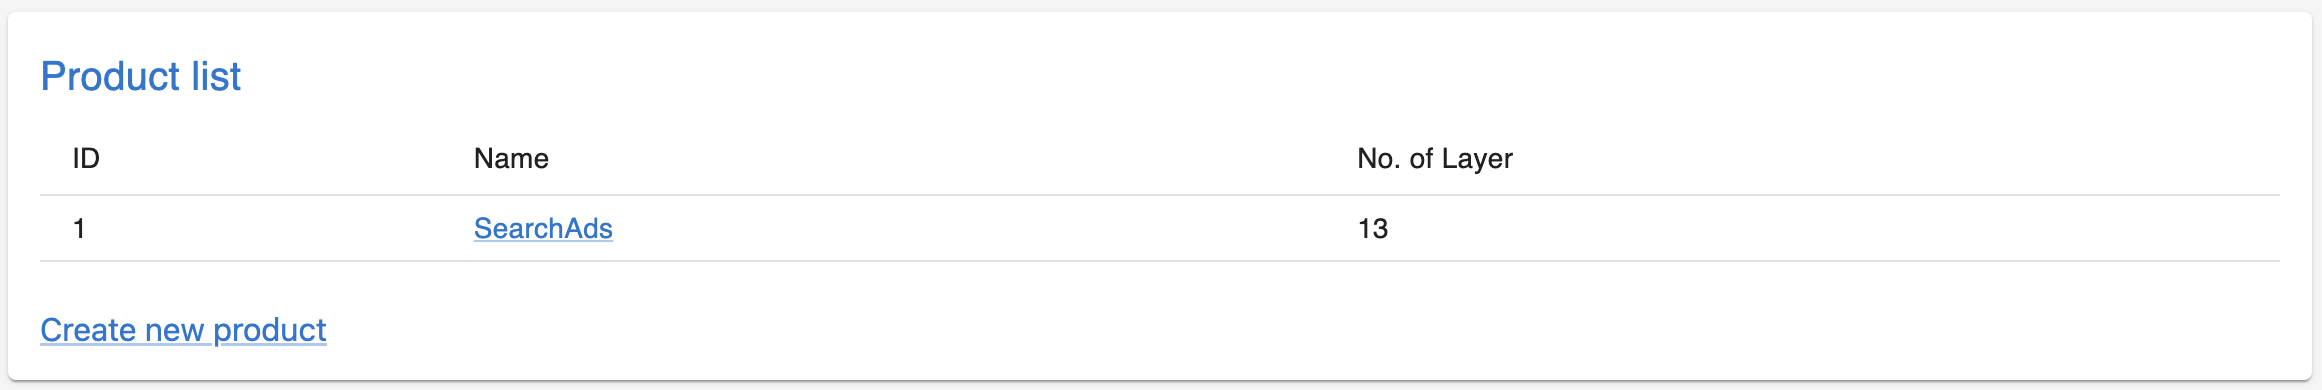
\includegraphics[width = 1\textwidth]{all-products}
	\caption{Tất cả Product}
\end{figure}

\subsubsection{Hiển thị thông tin của một Product}

\begin{figure}[H]
	\centering
	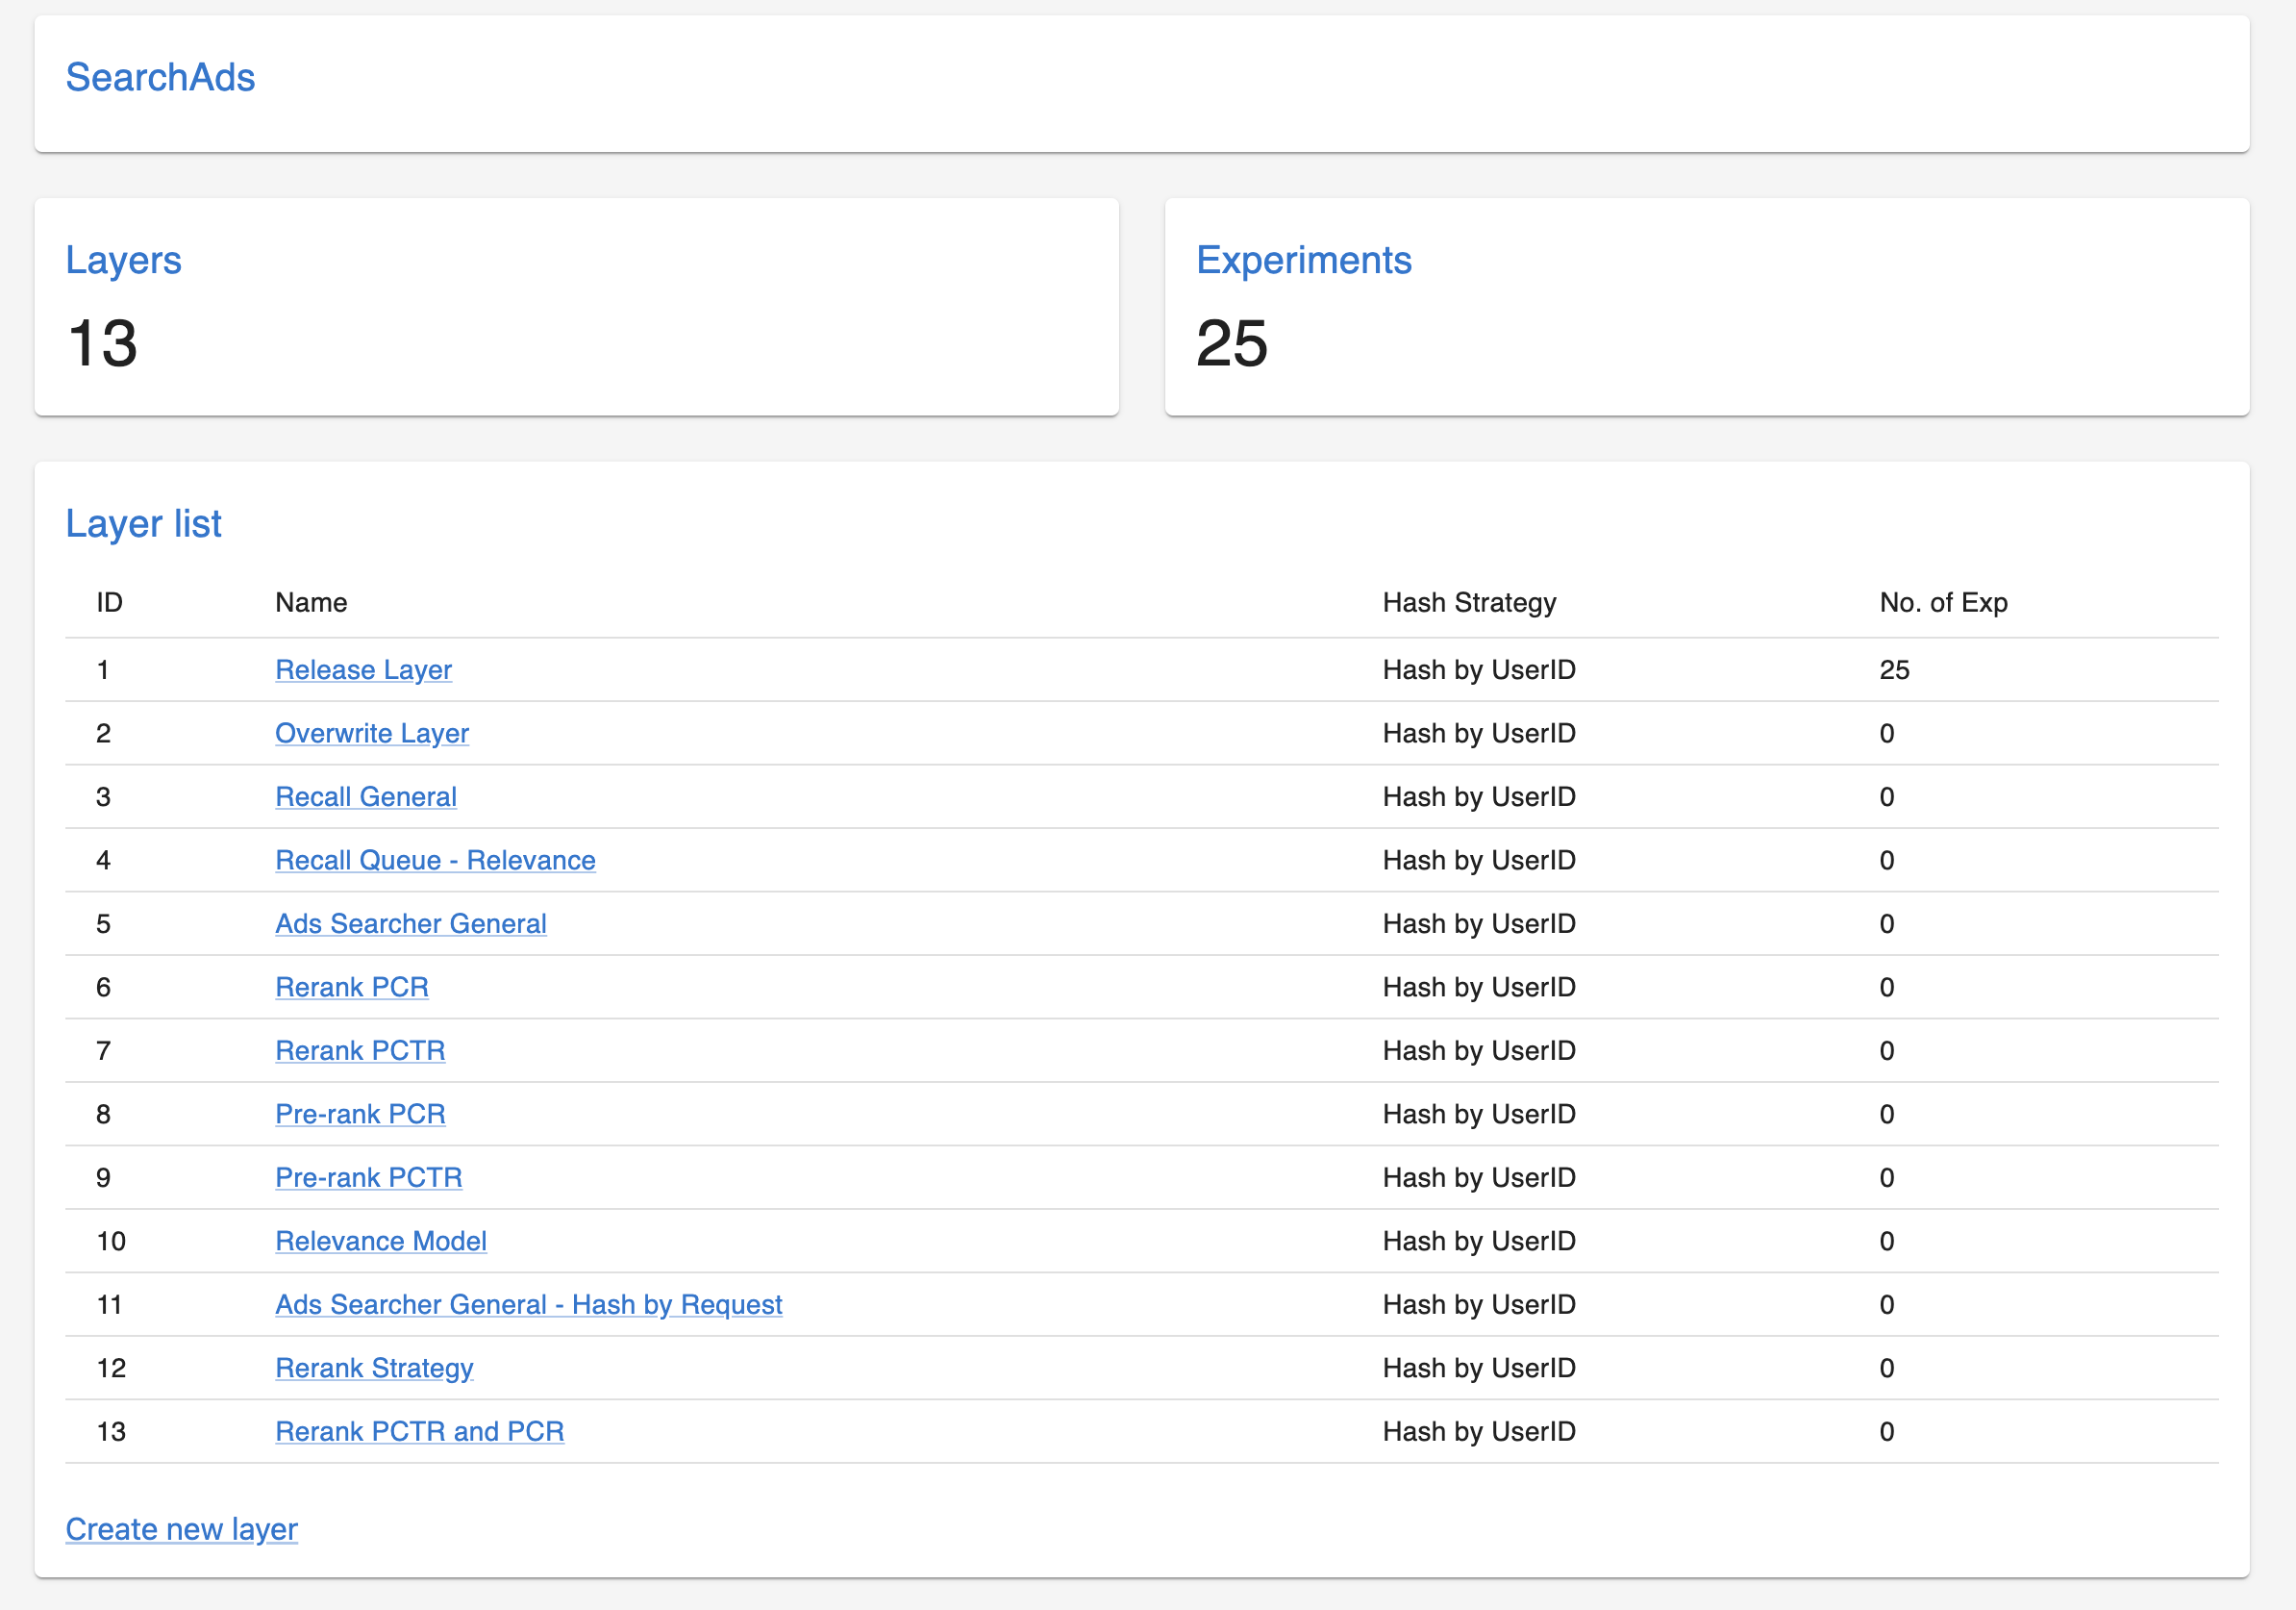
\includegraphics[width = 1\textwidth]{one-product}
	\caption{Thông tin của một Product}
\end{figure}

\subsubsection{Hiển thị thông tin của một Layer}

\begin{figure}[H]
	\centering
	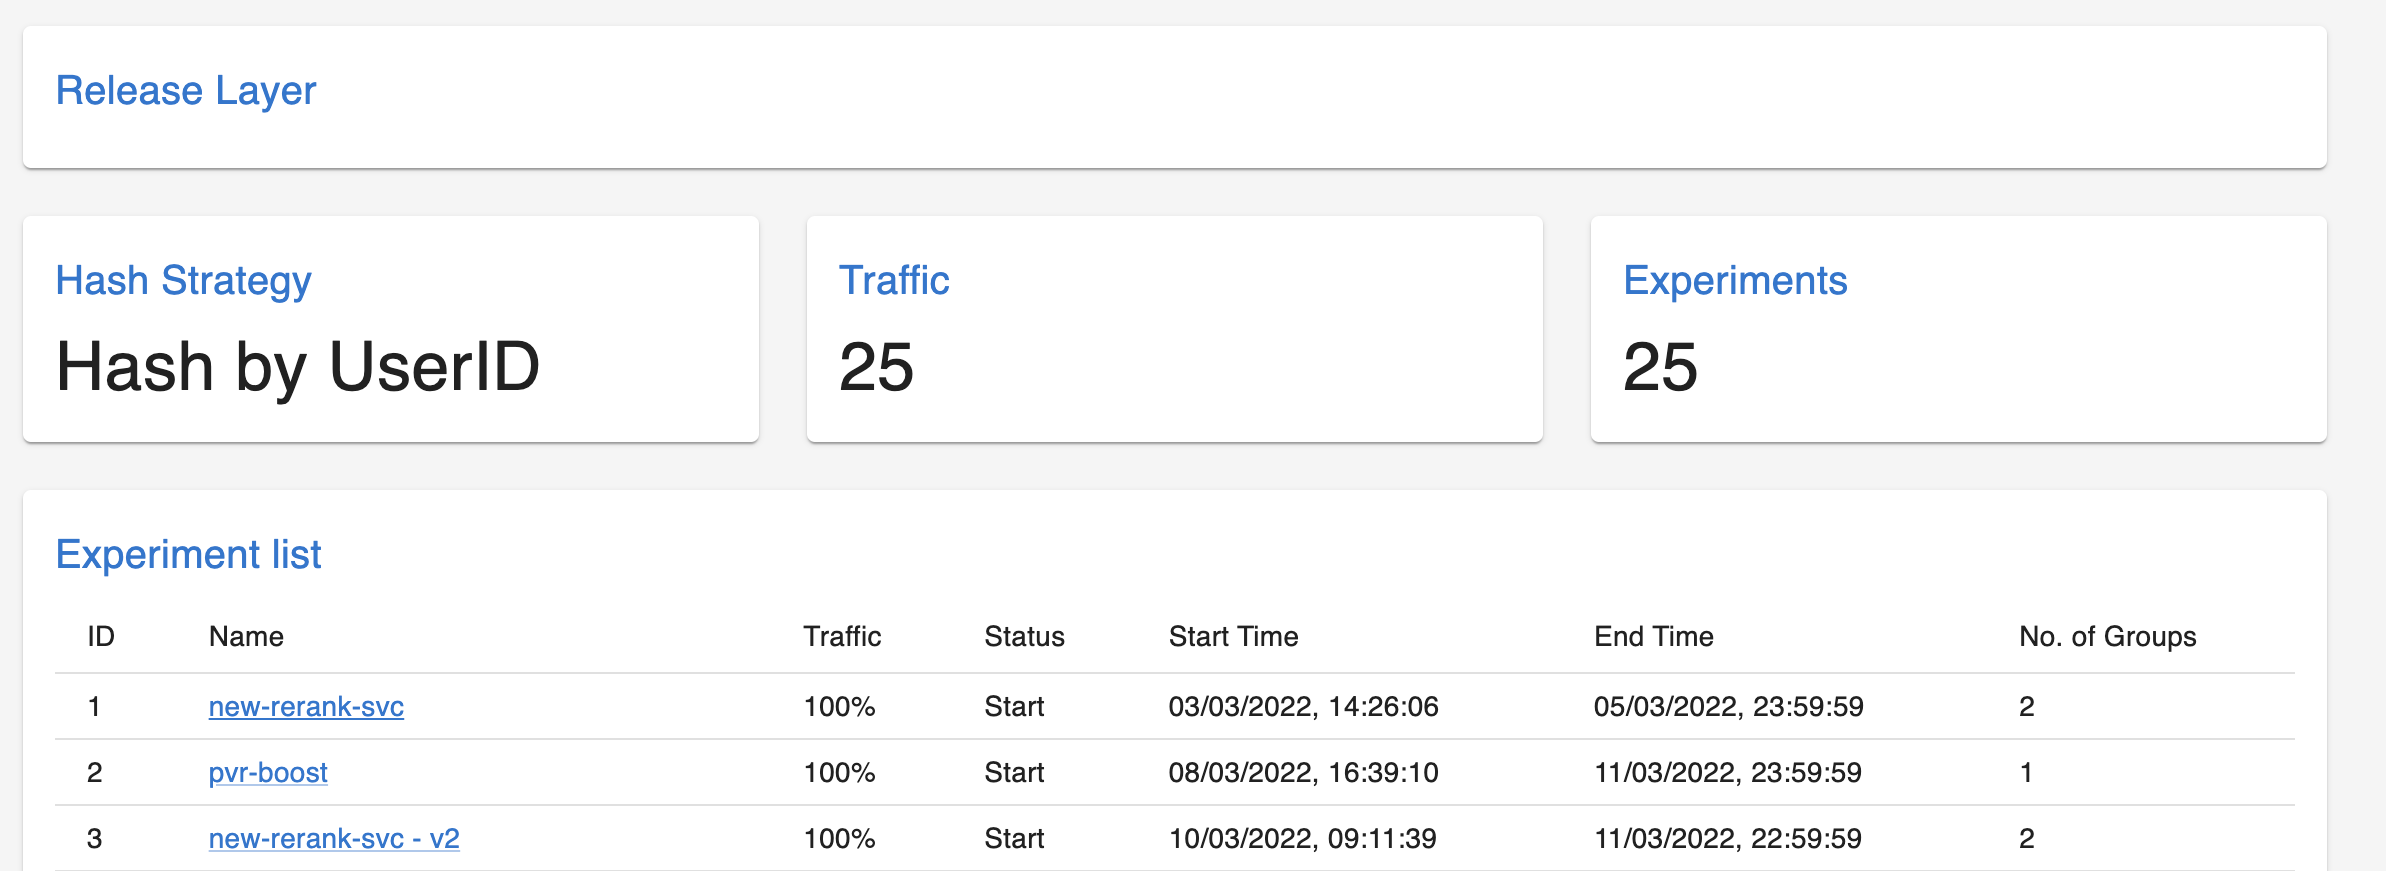
\includegraphics[width = 1\textwidth]{one-layer}
	\caption{Thông tin của một Layer}
\end{figure}

\subsubsection{Hiển thị thông tin của một Experiment}

\begin{figure}[H]
	\centering
	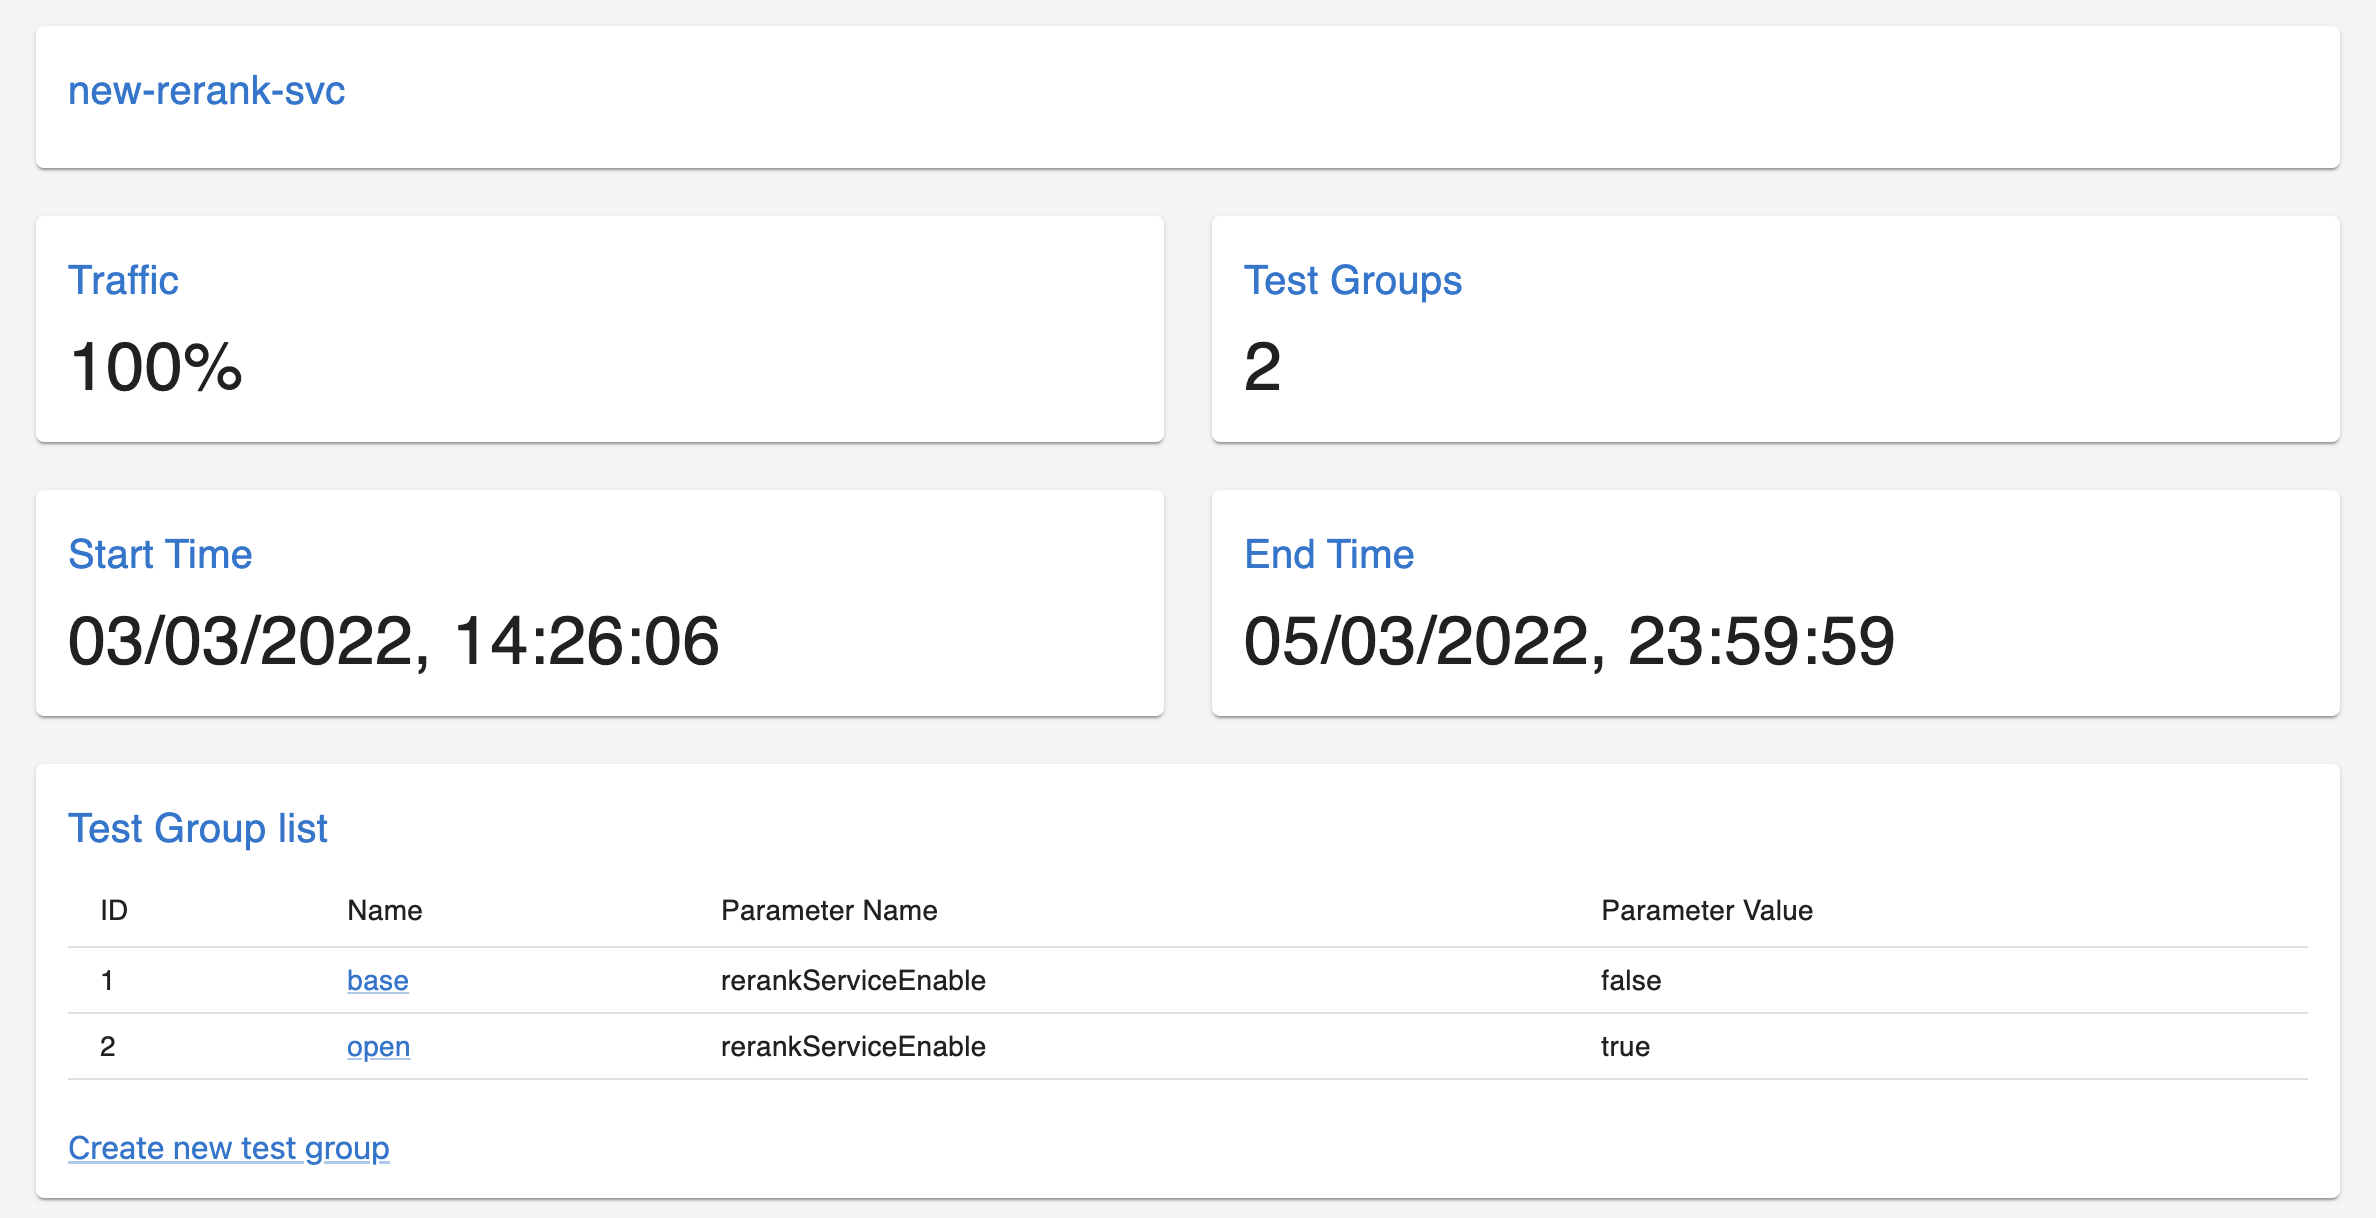
\includegraphics[width = 1\textwidth]{one-experiment}
	\caption{Thông tin của một Experiment}
\end{figure}
